\section{Fazit und Vision}

Im Verlauf des Projekts wurden Informationen aus den verschiedensten Bereichen zusammengetragen und in diesem Dokument destilliert. In den folgenden Abschnitten werden nochmals die Schlussbemerkungen eines jeden Abschnitts zusammengefasst.	 

\subsection{Bilanz in Bezug auf die Ist-Analyse zu Beginn des Projekts}

Zum Ende dieses Projekts soll diese Arbeit anhand der generierten Kennzahlen Tabelle \ref{tab:grad_der_digitalisierung}, aus dem Abschnitt \ref{sec:bilanz_des_projekts}, Bilanziert werden. Dafür wurde diese Tabelle aktualisiert. Das Resultat ist die Tabelle \ref{tab:grad_der_digitalisierung_upgrade}. Zu Beginn des Projekts hatte die Tabellenhälfte mit den MVT Versuchsständen, in der Spalte  \textbf{\textit{priorisierte} Einrichtungen}, einen prozentualen Anteil, relativ zu allen Spalteneinträgen, von 50~\%. Beim Projektabschluss wurde dieser Wert auf 100~\% angehoben. Folglich haben sich auch die prozentualen Anteile der Spalten \textbf{Sensorik vorhanden}; von 29~auf~43~\%; und \glqq \textbf{effektive Schnittstelle}\grqq; von 50~auf~67~\%; verändert. Die untere Tabellenhälfte, mit den MVT Analyseeinrichtungen, hat keine Veränderungen von sich getragen. \\





\begin{table}[p!] % Grad der Digitalisierung
\caption{\glqq Grad der Digitalisierung\grqq{} der MVT Geräte und Anlagen} \label{tab:grad_der_digitalisierung_upgrade}
\begin{center}
\begin{NiceTabular}{r|c|c|c|c}%[hvlines-except-corners=NW]
MVT Versuchsstände 			& 	\makecell{Sensorik\\ zweckmäßig} & \makecell{Sensorik\\ vorhanden} &  \makecell{\glqq effektive\grqq \\Schnittstelle}	& \makecell{\textit{priorisierte} \\Einrichtungen}  	 \\ \hline 
Sichten 								&						&	 			&  									&\\[0.2em]
Kuchenfiltration 					&		$\circ$		& 	\textcolor{OliveGreen}{\cmark}	&	\textcolor{OliveGreen}{\cmark} 	& \textcolor{OliveGreen}{\cmark}\\[0.2em]
Blaine								&						&			& 										&			\\[0.2em]
Staubabscheidung 				&		$\circ$		& \cmark			& \cmark							&  \cmark \\[0.2em]
Wirbelschicht 					&		$\circ$		&	\textcolor{OliveGreen}{\cmark} &	 \textcolor{OliveGreen}{\cmark} & \textcolor{OliveGreen}{\cmark}	 \\[0.2em]
Backenbrecher 					&						& 	 		& 										&\\[0.2em]
Planetenkugelmühle 			&		$\circ$		& \cmark	& 	 \xmark									&\\[0.2em]
Prallmühle 						&						&			& 										&\\[0.2em]
Walzenmühle						&						&	 		& 		&\\[0.2em]
Schneidmühle 					&						&  		& &\\[0.2em]
Hochdruckhomogenisator 	&						& 			& &\\[0.2em]
Intensivmischer 					&						& \cmark	& \xmark& \\[0.2em]
Conchiermaschine 				&						&			& & \\[0.2em]
Rührversuch 						&		$\circ$		&	\cmark		& \cmark	&   \cmark \\[0.2em]
\hline \hline
Summe aller~ \cmark,~\textcolor{OliveGreen}{\cmark}~oder~ $\circ$		&			5			& 4 					& 4    & 4 \\
Summe 	aller~ \xmark ~oder~ \textcolor{red}{\xmark}			&						&  	& 2    & 2\\[0.25em]
\makecell{prozentualer Anteil, relativ zu allen \\
\textcolor{black!50}{Einrichtungen} | Spalteneinträgen}	&	\textcolor{black!50}{36~\%}				&	\textcolor{black!50}{43 \%} 	 & 67~ \% & 100 \%\\[0.2em]

\Block{1-5}{} 						&			& 						& & \\[0.2em]
MVT Analyseeinrichtungen	&  \makecell{Sensorik\\ zweckmäßig}	&	\makecell{Sensorik\\ vorhanden} 	& \makecell{\glqq effektive\grqq \\Schnittstelle} & \makecell{ \textit{priorisierte }\\Einrichtungen} \\ \hline 
Zugversuch 						&	$\circ$	& \cmark 	& 	\cmark	&		\\[0.2em]
{Siebturmanalyse}\textsubscript{zzgl. digital Waage}				&	$\circ$	& \cmark 			& 		\xmark			&	\textcolor{red}{\xmark}	\\[0.2em]
Luftstrahlsiebung				& 	$\circ$	& \cmark 			& \cmark 		& \cmark \\[0.2em]
Scherzelle 							&	$\circ$	& \cmark 	&  \xmark 	& \textcolor{red}{\xmark}\\[0.2em]
Stampfdichte 					&		&  			&   									&\\[0.2em]
\makecell[r]{Laserbeugungs-\\
Partikelgrößenanalyse}					& 	$\circ$	& \cmark 			&  \cmark 							& \cmark\\[0.2em]
\hline \hline
Summe aller~ \cmark ~oder~ $\circ$							&	5	& 4 					& 2	&	2		\\
Summe 	aller~ \xmark ~oder~ \textcolor{red}{\xmark}	&		&  					& 2	&		2	\\[0.25em]
\makecell{prozentualer Anteil, relativ zu allen \\
\textcolor{black!50}{Einrichtungen} | Spalteneinträgen} 			& \textcolor{black!50}{83~\%}	&	\textcolor{black!50}{83 \%} 		& 60 \% 						& 50~\%	\\[0.2em]
\end{NiceTabular}
\end{center}
\end{table}

\FloatBarrier 

\subsection{Fazit und Vision des Kapitels Konzeptentwicklung}

Das verfahrenstechnische Labor soll zeitgemäß, digital transformiert werden. An der Stelle muss nochmals erwähnt werden, dass eine digitale Transformation ein Prozess und kein Projekt ist. Das Konzept 3.0, ohne Datenbankmanagementsystem (DBMS), sollte als Vorstufe des Konzept 4.0, mit DBMS, betrachtet werden. Das Konzept 3.0 ist eine Mindestanforderung für die digitale Transformation des verfahrenstechnischen Labors. Im folgenden werden die Wünsche und Anforderung aus dem Kapitel \ref{sec:konzeptentwicklung} {\Hypatia Konzeptentwicklung für die Labordigitalisierung} aufgelistet. Die erfüllten Anforderungen werden mit einem Haken (\cmark) und die Anforderungen, die im Rahmen dieses Projekts nicht umgesetzt wurden, mit einem Kreuz (\xmark) markiert. Stichpunkte, die Anmerkungen enthalten, werden mit einem $\diamond$ gelabelt. 

\begin{enumerate}[leftmargin = 1.5em, label = \textbullet , itemsep = 0.1em]
\item[\cmark] Das Konzept soll für das verfahrenstechnische Labor allgemeingültig sein.
\item[\cmark] Die \glqq \,{\Menlo digitalen Kompetenzen}\grqq{} der Studierenden sollen maximiert werden, ohne die fachlichen Kompetenzen signifikant zu reduzieren, durch 


	\begin{enumerate}[leftmargin = 1.5em, label = -- , itemsep = 0.1em]
	\item[\cmark] ein Minimum an Automatisierung 
	\item[\cmark] Unter Automatisierung kann z.B.  die Manipulation von Daten, wie die Detektion von Ausreißer und dessen Entfernung, genaue Leitfäden in der Handhabung, die keine Fehler mehr zulassen o.ä., verstanden werden.
	\end{enumerate}
	
\item[\cmark] Der monetäre Aufwand soll minimal sein.
\item[\cmark] Möglichkeiten der Datenerfassung/Signalverarbeitung sollen eruiert werden. 
\item[\cmark] Die inkrementelle Implementation von Applikationen im Rahmen von Industrie 4.0 und Big Data (KI, Digital Twin etc.) soll tendenziell möglich sein.
	\begin{enumerate}[leftmargin = 1.5em, label = $\diamond$ , itemsep = 0.1em]
	\item Es wurden keine Schritte eingeleitet, die eine inkrementelle Implementation von Applikationen ausschließen.
	\end{enumerate}


\item[\cmark] Cloud Computing soll in Betracht gezogen werden.

	\begin{enumerate}[leftmargin = 1.5em, label = $\diamond$ , itemsep = 0.1em]
	\item Die Implementation eines Cloudservice (HAW Cloud) ist im Verlauf des Projekts nicht erfolgt. Im Verlauf eines Telefonats mit einem ITSC-Mitarbeiter am 08.02.21, um ca. 11 Uhr, scheinen die HAW Richtlinien es \textbf{derzeit} nicht zu gestatten, dass Kennungen an nicht humane Entitäten bzw. nicht natürliche Personen vergeben werden (siehe Protokoll im Anhang \ref{appendix:Cloudnutzung1} und \ref{appendix:Cloudnutzung2}). Die HAW-Cloud funktioniert nutzerbezogen, wofür Kennungen (des Typs axxXXX) erforderlich sind. Nicht humane Entitäten könnten die folgenden sein:
	 
		\begin{enumerate}[leftmargin = 1.5em, label = -- , itemsep = 0.1em]
		\item Aggregate
		\item Maschinen
		\item Geräte
			\begin{enumerate}[leftmargin = 1.5em, label = - , itemsep = 0.1em]
			\item HMI's 
			\item Sensoren
			\end{enumerate} 
		\end{enumerate}
	\end{enumerate}
	
	\begin{enumerate}[leftmargin = 1.2em, label = -- , itemsep = 0.1em]
	\item[\xmark] Erster Schritt der Umsetzung: Speicherung der Rohdaten auf der HAW Cloud
		\begin{enumerate}[leftmargin = 1.2em, label = $\diamond$ , itemsep = 0.1em]
		\item Da die Nutzung der HAW Cloud möglich wäre, der Aufwand dem Nutzen jedoch nicht gerecht wird, wurde eine alternative Lösung entwickelt  (siehe Anhang  \ref{appendix:Cloudnutzung1},\ref{appendix:Cloudnutzung2}). Als Alternative  wurde ein lokaler Server an der HAW Life Sciences, am Standort Bergedorf vorgeschlagen.
		
		\end{enumerate} 
	\item[\xmark] Zweiter Schritt der Umsetzung: Cloudnutzung, gemäß des Impulsvortrags zum Digitalisierungsfond $\Rightarrow$ Amazon, Google, Microsoft Azure
	\end{enumerate}
	
\item[\xmark] Die gesamte Protokollierung der Studierenden soll in Zukunft digital sein.

	\begin{enumerate}[leftmargin = 1.5em, label = $\diamond$ , itemsep = 0.1em]
	\item Der Fortschritt des Teilprojekts, unter der Leitung von Dipl.-Ing. M. Hannappel und Dipl.-Ing. S. Wittkowski, \textit{Electronic Labor Notebook} hat noch keine vollständige Validierung des Konzepts 3.0 zugelassen.
	\end{enumerate}

\end{enumerate}

%Eine Lösung der Signal- bzw. Datenverarbeitung wurde generiert, dafür wurde die Applikation LabVIEW des Unternehmens National Instruments genutzt. Die Wirbelschichtversuchsanlage sowie die Filterkuchenversuchsanlage wurden mit LabVIEW abgebildet. Dafür wurde das Datalogging von diskreten sowie kontinuierlichen Daten ermöglicht. In den in LabVIEW programmierten Applikationen einen Speicherpfad auf einen lokalen Server zu realisieren, war im Verlauf des Projekts noch nicht möglich.  \\


Der \textit{digitale Transformationsprozess} des verfahrenstechnischen Labors wurde mit dem Konzept 3.0 initialisiert. Die \textbf{{\Hypatia Vision}} sollte die inkrementelle Umsetzung des \textbf{{\Hypatia Konzepts 4.0}} sein (siehe Abbildung \ref{digitalisierungskonzept_mit_db}). Meines Erachtens nach unterliegt der Aufwand dem Nutzen der Realisierung des Konzepts 4.0  im hohem Maße, aus den folgenden Gründen. \\

Im akademischen Rahmen unterliegt der Aufwand, der Realisierung des {\Hypatia Konzept 4.0}, einen \textbf{großen} Mehrwert, in Bezug auf das Verständnis und Lernerfolg der Studierenden. Die Datenbank könnte auch für den Laborbetrieb des Departments genutzt werden, wodurch sich möglicherweise organisatorische Vereinfachungen, wie z.B. Chemie- und Verfahrenstechniklagerverwaltung o.ä. realisieren lassen. Des Weiteren könnte die Datenbank für die verfahrenstechnische Forschung, Projekte im Rahmen der angewandten numerische Simulation, uvm. genutzt werden. Die \textbf{größte Hürde} für die {\Hypatia Konzept 4.0} Realisierung könnte der \textbf{Changeprozess} sein, daher wurde der Punkt Changeprozess, in der Tabelle \ref{tab:konzept4.02} mit einem Dicken \textbf{Minus} (--) versehen.\\

In unserer agitierten Welt ist weder Platz für schwere Unternehmenstanker noch für träge Universitäten oder Hochschulen. In der Zeit der Globalisierung und digitalen Transformation ist Flexibilität und Vernetzung nicht nur eine hinreichende Forderung, sondern absolut notwendig. Unternehmen sollten sich Ihre Spitzenkräfte schaffen. Der Spruch, \glqq von der Berufsausbildung oder dem Studium braucht man am Ende des Tages maximal 15 \%\grqq , ist nicht tolerierbar sowie zu verantworten und doch ist es aus eigenen Erfahrungen Realität. Wie lange Überlebt ein Unternehmen welches 85 \% Ausschuss hat? Wenn durch diese Art des Paradigmenwechsels eine Ausschussreduktion auf bspw. 70 \% erfolgt, ist das ein immenser Fortschritt! 
In der Tabelle \ref{tab:konzept4.02} sind die Vor- und Nachteile des Konzepts 4.0 nochmals aufgelistet.\\

\begin{table}[h!]
\caption{Vor- und Nachteile des Konzeptentwurfs 4.0} \label{tab:konzept4.02}
\centering
\vspace{1em}
\begin{tabularx}{1\textwidth}{X|X}
Vorteile & Nachteile \\ \toprule \vspace{-1,5em}
\begin{itemize}[leftmargin=*,labelsep=-\mylen]
\item[+] Stand der Technik in der Industrie	/ Zeitgemäß 
\item[+] Nutzbar für Tätigkeiten außerhalb vom VT1 und VT2 Praktikum (Forschung, Organisatorisches 
wie 
\item[+] Lagerverwaltung, angewandte numerische Simulation	uvm.)
\item[+] wenn Cloudservicenutzung, dann Port\-folio\-software Kompatibilität des \mbox{Anbieters}
\item[+] Image/Professionalität (u.a. auch Anmerkungen von Bachelorabsolventen Ende 2020)
\item[+] ggf. mehr Kooperationsprojekte mit Unternehmen und Universitäten
\item[+] Kompetenzsteigerung der Hochschule und Absolventen
\item[+] interdisziplinäre Vernetzung/Projekte  (Industrie 4.0 $\equiv$ Vernetzung)
\item[+] gute Investigationsmöglichkeiten bei Produktabweichung bei konstanten Parametern $\rightarrow$ Studentenprojekte
\end{itemize}
\vspace{-1,5em}
&
\vspace{-1,5em}
\begin{itemize}[leftmargin=*,labelsep=-\mylen]
\item[--] Changeprozesse
\item[-] notwendiges Know-How erforderlich
\item[-] Aufwand der Erstellung der Datenbank
\item[-] Einrichtung automatischer Einspeisung der Sensordaten in die Datenbank
\item[-] Kosten könnten entstehen
\begin{itemize}[leftmargin=*,labelsep=-\mylen] 
\item[\textbullet] möglicherweise Sponsoring/Kooperation (als Gegenleistung Projekte o.ä) da Hochschule 
\item[\textbullet] geringe Datenmengen im vgl. zu Unternehmen $\rightarrow$ möglicherweise keine oder geringe Kosten
\end{itemize}
\end{itemize}
\end{tabularx}
\end{table}

Im Rahmen der Anwendungsfälle im Hochschulalltag könnten SQL Datenbanken den Anforderungen genügen. Das Know-How mit dieser standardisierten Datenbanktechnologie ist auf andere Softwaretechnologien transferierbar.  Es sollte auch möglich sein, die Erstellung einer Datenbank, im Rahmen studentischer Arbeiten, zu delegieren. Des Weiteren ist auch im Verlauf des \textit{Digitalisierungsprozess} eine Hybridlösung denkbar. Datenbankmanagement könnte \,{\Menlo Morgen}, in diesem \,{\Menlo digitalen} \,{\Menlo Zeitalter}, eine von Ingenieuren geforderte \textbf{{\Hypatia Kernkompetenz}} sein.

\FloatBarrier 
\pagebreak
\subsection{Fazit und Vision des Kapitels Signalverarbeitung}

Zu Beginn des Projekts wurden Anforderungen an die Signalverarbeitung definiert. Erfüllte Anforderungen werden ebenfalls mit einem Haken (\cmark) und nicht erfüllte mit einem (\xmark) versehen.

\begin{enumerate}[leftmargin = 1.5em, label = \textbullet , itemsep = 0.1em]
\item[\cmark] Die Applikationen sollen eine graphische Oberfläche haben.
\item[\cmark] Der Aufwand für die Applikationsgenerierung soll minimal sein.
\item[\cmark] Die Applikationen sollen nur von ausgewählten Personal (\glqq leicht\grqq{}) anpassbar sein.

\begin{enumerate}[leftmargin = 1.5em, label = \textbullet , itemsep = 0.1em]
\item[$\diamond$] Den wissenschaftlichen Mitarbeitern ist das Passwort bekannt (Entsperrungssequenz bspw. durch Druck der Kombination Strg+E zu erreichen)
\end{enumerate}

\item[\cmark] Die verwendete Software soll in der Lage sein, Daten der verschiedenste Versuchsstände und Geräte unterschiedlicher Hersteller abzubilden.
\item[\cmark] Es sollen Echtzeitgraphen generiert werden können.
\item[\cmark] Die verwendete Applikation soll kontinuierliche und diskrete Daten verarbeiten können.
\item[\cmark] Die Möglichkeit, die Daten in Zukunft direkt in eine Datenbank schreiben zu können, ist wünschenswert.

\begin{enumerate}[leftmargin = 1.5em, label = \textbullet , itemsep = 0.1em]
\item[$\diamond$] Es ist möglich die Daten via LabVIEW direkt in eine Datenbank schreiben zu lassen.
\end{enumerate}

\item[\textcolor{OliveGreen}{\cmark}] Im Verlauf des Projekts wurde ein Schreibschutz der Datein nach Abschluss  eines Versuchsdurchgangs erwünscht. Dieser Wunsch wurde erfüllt. 

\begin{enumerate}[leftmargin = 1.5em, label = \textbullet , itemsep = 0.1em]
\item[$\diamond$] Das kopieren der Daten aus der Datei und Löschen der Datei ist weiterhin möglich. Eine Manipulation kann derzeit durch den Speicherungszeitpunkt der \textbf{neuen} Datei und ob ein Schreibschutz bei der \textbf{neuen} Datei aktiviert wurde ermittelt werden.
\end{enumerate}
\end{enumerate}

Es wurde ein Programm mittels Python geschrieben und ist als .py Datei dem Anhang beigefügt. Es ist in der Lage eine RS-232 Waage \,{\Menlo auszulesen}, die Werte zu \,{\Menlo interpretieren} und einen \,{\Menlo Graphen} zu \,{\Menlo plotten} (siehe Abbildung \ref{fig:Gravimetrischemessung_python}). \\

\begin{figure}[h!] %[htbp!] 
\centering
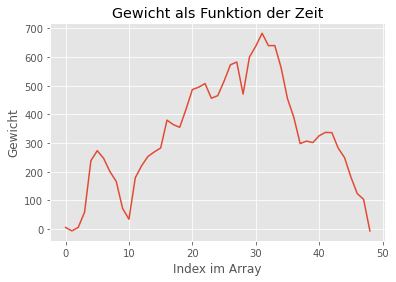
\includegraphics[width=0.5\textwidth]{Bilder/Gewicht_als_Funktion_der_zeit.png}
\vspace{0em}
 \caption[Gravimetrische Messung in Python]
{Gravimetrische Messung in Python}\label{fig:Gravimetrischemessung_python}
\end{figure}

Da die Implementation eines Cloud oder lokalen Servers nicht erfolgt ist, werden die Datalogs derzeit auf dem jeweiligen Laborrechner auf dem Desktop gespeichert. Der Dateipfad ist bei nachträglicher Implementation von Serverlösungen in den VI`s, in der Initialisierung anzupassen (siehe Abbildung \ref{fig:schreibschutz_dialog} im Abschnitt \ref{sec:Pfad}).\\

Die Idee, dass jeder Laboraccount eine eigene Kennung erhält, wodurch die Laborgeräte wie HMI's ein Cloudverzeichnis auf der HAW Cloud erhalten würden, ist derzeit nicht realisierbar. Die Idee, dass nicht humane Entitäten eine Kennung erhalten können, sollte in höheren Instanzen der HAW diskutiert werden, damit zukünftige Cloudlösungen HAW global realisiert werden können. Die Hochschule sollte das Ziel haben die Privatwirtschaft abzubilden. Das nicht humane Entitäten ein eigenes Kommunikationbsnetzwerk erhalten ist bereits Stand der Technik (siehe Abschnitt \ref{sec:bluetooth}). \\

Es ist anzumerken, dass die in LabVIEW geschrieben Programme alle Daten in einer \,{\Menlo *.txt} Datei als Strings speichern. Bei einem Import ist eine Umwandlung zu erfolgen ( in bspw. Excel \,{\Menlo Zellen} \,{\Menlo formattieren..}). Es wird empfohlen den Studenten dass \textbf{nicht} mitzuteilen, damit ein autodidaktischer Lernprozess stattfinden kann.




\subsection{Fazit und Vision der Teilumsetzung an den ausgewählten Versuchsanlagen}


Die Filterkuchen- sowie die Wirbelschichtversuchsanlage wurde mit geeigneter Sensorik aufgerüstet, um die kontinuierlichen Parameter, Druck $p$ und Volumenstrom $\dot{V}$, zu erfassen. Des Weiteren wurde neben dem Datalogging kontinuierlicher Parameter, das Datalogging diskreter Daten ermöglicht. Die Messspanne der Drucksensoren ist von -1~bis~1~bar relativ zur Atmosphäre; repräsentiert von der elektrischen Signalspanne von 0~bis~10~V; und die des thermischen Massen\-durchfluss\-sensors an der Wirbel\-schicht\-versuchsanlage ist von 0~bis~50~l/min; repräsentiert durch die elektrische Signalspanne von 4~bis~20~mA.\\

Eine digitale Erfassung der Festbett- bzw. Wirbelschichthöhe an der \textbf{{\Hypatia Wirbelschichtversuchsanlage}} ist denkbar. Bei Bedarf könnten bspw. geeignete optische, akustische, mechanische Entfernungsmesser, im Rahmen einer studentischen Projektarbeit, recherchiert und ggf. umgesetzt werden. Eine Implementation in die im Rahmen dieser Arbeit programmierten Applikation sollte komplikationslos möglich sein. Des Weiteren könnte die Steuerung des Volumenstroms, derzeit per Handventil, durch eine digitale Steuerung ersetzt werden. Der derzeitige Volumenstromsensor (VA-525) könnte dadurch substituiert und für andere Versuchsaufbauten verwendet werden.\\

Die \textbf{{\Hypatia Filterkuchenversuchsanlage}} hat eine umfangreichere Funktion der diskreten Datenaufnahme erhalten. Die Feststoffbestimmung im Filtrat kann manuell im LabVIEW Programm dokumentiert werden. Diese Messverfahren ist eine Vergleichsmessung mit der Bezeichnung \textit{Tubidimetermessung}. Neben der Datalogdatei der kontinuierlichen Messung, 
die ebenfalls den Header enthält, analog der Wirbelschichtversuchapplikation, wird eine zweite Datei generiert. Die Funktionsweise der Datalogger werden in den folgenden Paragraphen nochmals zusammengefasst.


\paragraph*{Kontinuierlicher Datalogger} 

Bei beiden Anlagen werden kontinuierliche Dateien des Typs\\ {\Menlo \,FK\_<Gruppen\_ID>.txt} und {\Menlo \,WS\_<Gruppen\_ID>.txt} generiert. Bei Starten einer Messung in der jeweiligen LabVIEW Applikation ist das Starticon $\Rightarrow$ oben links im {\Hypatia Front Panel} zu betätigen. Es folgt ein Dialogfenster, wo der Dateiname des Typs, wie oben Angegeben, eingegeben werden soll. Ist vor dem Applikationsstart bereits die {\Menlo Gruppen\_ID} eingegeben worden, dann ist nur das suffix {\Hypatia .txt} zu ergänzen. Ist vor dem Applikationsstart bereit die {\Menlo Gruppen\_ID} eingegeben worden, dann ist nur das suffix {\Hypatia *.txt} zu ergänzen. Bei beiden Dataloggern wird im Falle einer redundanten Namensvergabe der Inhalt der nächsten Versuchsiteration unten dem Dokument angehängt. Ein Datenverlust ist ausgeschlossen. Im Verlauf des Projekts wurde sich ein Schreibschutz der Datalog-Datei gewünscht. Die LabVIEW Applikation kann die Verschlüsselung wieder öffnen das Logging am Dokumentende starten und am Ende wieder Verschlüsseln. 

\paragraph*{Diskreter Datalogger}
Die Applikation der Filterkuchenversuchsanlage generiert zwei Dateien. Bei Starten einer Messung in der Applikation {\Menlo Filterkuchenversuch\_V01DL.vi}, durch das Betätigen des StartIcons ($\Rightarrow$)  oben links im {\Hypatia Front Panel}, folgen zwei Dialogfenster, wo der Dateiname des Typs, wie oben Angeben, eingegeben werden soll. Beim zweiten Dialogfenster, für die Tubidimeter Datei ist eine analoge Dateinamenvergabe zu vollziehen ({\Menlo FK\_Tubi\_<Gruppen\_ID>.txt}). \textbf{Bei dieser Datei wird die Datei Überschrieben!} Der Grund liegt an der Tatsache, dass bei der Filterkuchenversuchsanlage drei Versuchsdurchläufe durchgeführt werden. Nach dem Beenden einer kontinuierlichen Messung werden die diskreten Tubidimeterspezifischen Daten eingebeben. Daraufhin wird bis zu dreimal der Versuch wiederholt. Die Tubidimeter Datei wird bei jeder Iteration weiter vervollständigt. Ein Anhängen der neuen Daten hätte sinnlose redundante Datengenerierung zur Folge. \textbf{Nach der letzten Iteration ist das Programm nochmals zu starten und mit Stop zu quittieren, da sonst die Tubidimeterdaten der letzten Eingabe nicht erfasst werden.} 

\paragraph*{Hinweis zum Schreibschutz}
Der gewünschte Schreibschutz der Dateien wurde implementiert, somit sind diese originalen Dateien nicht modifizierbar, jedoch ist das Kopieren und das Einfügen des Inhalts in eine andere Datei weiterhin möglich. Des Weiteren beinhaltet der Schreibschutz nicht das nicht Löschen der Datei. Manipulationsversuche können somit nur damit detektiert werden, wann die Datei erstellt wurde und ob ggf. ob kein Schreibschutz bei einer duplizierten und manipulierten Datei vorhanden ist oder nicht. \\



Abschließend kann gesagt werden, dass der erste Schritt der \textit{digitalen Transformation} getätigt wurde. Es war mir eine Ehre den ersten Schritt beitragen zu dürfen. Ich wünsche der HAW Life Sciences viel Erfolg für die nächsten Schritte.
